\chapter{Porting Contiki \gls{os} to a \gls{ble} platform} \label{5bleContiki}

This chapter describes the initial task of choosing the hardware platform supporting \gls{ble} and porting Contiki \gls{os} to this platform. This task was a pre-requisite to the next task of testing detailed in chapter \ref{6Testing}. Section \ref{5HwPlt} explains the process of choosing a hardware platform and describes the chosen one. Section \ref{5Porting} describes the different aspects of porting Contiki to a new platform, with details of the specific port done in this project.

\section{\gls{ble} Hardware Platform} \label{5HwPlt}

As mentioned in section \todo{ref{4Porting}} Contiki has been ported to many hardware platforms. Since one of the main feature of Contiki is its communication stack capable of running in resource constrained systems, the primary aspects of a hardware platform are the \gls{mcu} and the communication interface. When choosing a hardware platform there are many other aspects that need to be considered as well. These include the availability of source code for peripheral drivers and examples, development environment (compiler, linker, programmer and debugger), development boards, documentation of the entire system and online forum for discussion.

There are two types of platforms, namely platforms which consist of circuit board with a discrete radio transceiver with a \gls{mcu} controlling it and platforms which consist of a \gls{soc} containing both the \gls{mcu} and radio transceiver in the same \gls{ic}. For including \gls{ble} support in Contiki, a hardware platform needed to be chosen and this process is explained in this section.

\subsection{Requirements of the hardware platform}
The \emph{mandatory} requirements for the platform would be:
\vspace{5pt}
\begin{easylist}[itemize]
& Must have a well supported and documented processor with good specifications.
& Availability of well documented datasheet and user manual.
& Availability of an evaluation/development kit.
& Enough memory to accommodate Contiki and \gls{ble} stack’s requirements.
& Presence of basic peripherals such as timers and serial port required for Contiki.
\end{easylist}
\vspace{10pt}
\noindent
The non-mandatory, although \emph{nice to have} requirements for the platform would be:
\vspace{5pt}
\begin{easylist}[itemize]
& A \gls{soc} based platform. A \gls{soc} solution is preferred  because of characteristics such as lower power consumption, lower circuit board area and lower total cost.
& For an open source project such as Contiki, a free and preferably open source development toolchain must support the platform.
& Presence of flexible power modes with low active and sleep power consumption.
& Availability of a good set of peripherals.
& Availability of \gls{ble} stack from the vendor, preferably with source code.
\end{easylist}
\vspace{10pt}

\subsection{Comparison and selection of the hardware platform}

With these requirements, based on the exhaustive comparison in Appendix \ref{ApdxSoC} of the available \gls{soc} (\gls{ble}+\gls{mcu}) solutions available today, a platform based on nRF51822 from Nordic-Semiconductors would be a suitable option. As seen from the table in Appendix \ref{ApdxSoC}, this platform would satisfy all the requirements mentioned above except for that the \gls{ble} stack would be available as a binary file, without the source code.

As shown in the table in Appendix \ref{ApdxSoC}, recently many new promising \gls{ble} based \glspl{soc} have be released such as Quintic 9020, Dialog Semiconductor DA14580, Lapis MLA7105 and Broadcom BCM20732. From the limited technical information available about them, their technical specifications would be suitable for a project like this. But because of the limited documentation about them, scarce availability and nascent support they are not suitable.

\subsection{Overview of nrf51822 \gls{soc} and its platform} \label{5nrfPCA}

nrf51822 is a \gls{soc} made by Nordic Semiconductor for developing \gls{ble} and 2.4 GHz based wireless systems \cite{nrf51822page}. Most of the specification of this \gls{soc} can be found in the table in Appendix \ref{ApdxSoC}. The ARM Cortex M0 present is a 32 bit, 3 stage pipeline processor with Von Neumann architecture. It is designed for low silicon die size, low cost and power. It has an integrated \gls{nvic}  responsible for handling processor exceptions and peripheral interrupts. 

The development boards in the form of a USB dongle used for this thesis are called PCA10000. As seen in the figure \ref{pca10000}, the top side of PCA10000 contains nrf51822 at the centre, powered from the USB port through a voltage regulator. This \gls{soc} is connected to a tri-colour RGB led, a 16 MHz crystal, a 32.768  kHz crystal and a PCB antenna with its matching network. On the other side of the PCB is the SEGGER JLink Lite Cortex M unit. This can program and debug using the Serial Wire Debug (SWD) port of nrf51822. Another useful feature of this board is that the SEGGER JLink unit provides a serial port over USB with hardware flow control (HWFC) to the computer that this dongle is connected to. This serial port is connected to the \gls{uart} port of nrf51822 \cite{PrithviR}.

\begin{figure}[h]
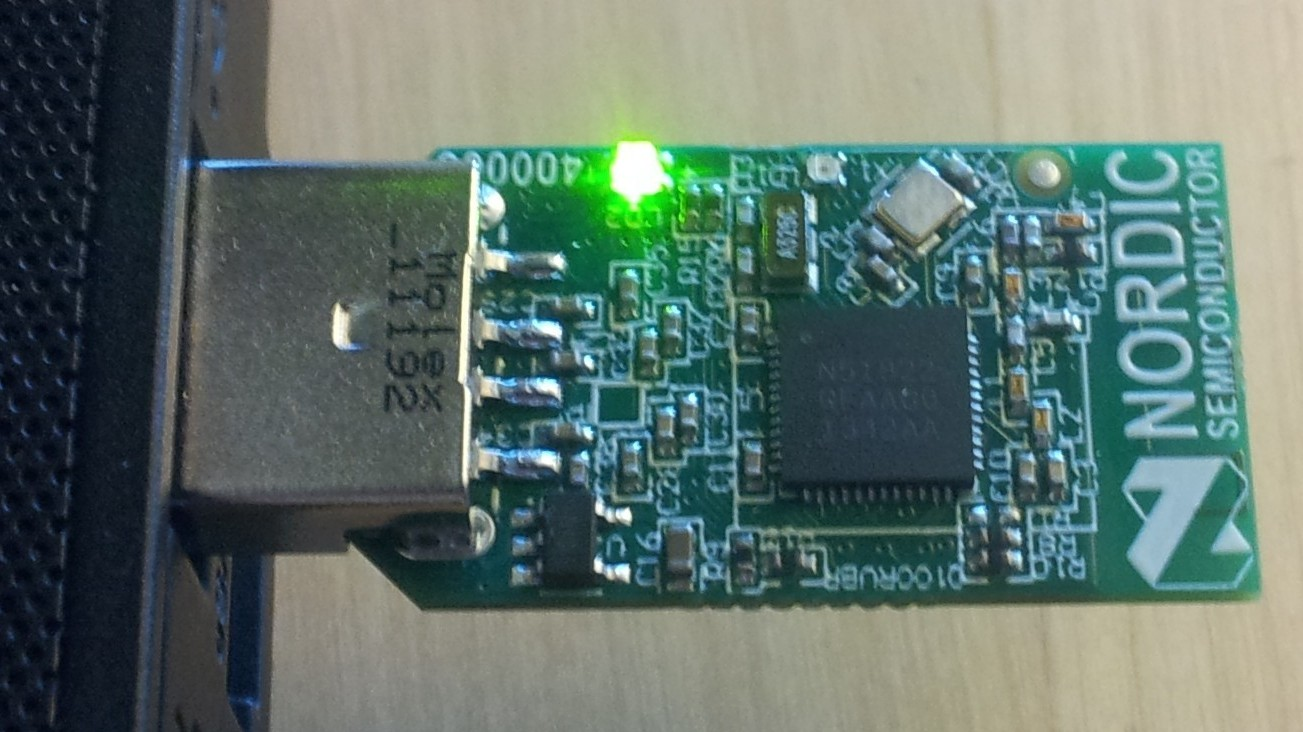
\includegraphics[width=\textwidth]{PCA10000}
\caption{PCA10000 development board}
\label{pca10000}
\end{figure} 

Nordic Semiconductor provides \gls{ble} stack as a precompiled and linked binary file called \emph{SoftDevice}. There are various of these SoftDevice binaries with different aspects of the \gls{ble} stack. The SoftDevice is stored in a protected area in the flash memory and has access to a protected section of \gls{ram} memory, preventing unauthorized access by the application code. The SoftDevice can be accessed through a specified set of \gls{api} calls. These \glspl{api} are accessed by making a supervisor call to the processor causing a exception handler to run the SoftDevice. All calls are non-blocking, which means that the call will not stall the application making the call. And there are synchronous and non-synchronous calls, where the synchronous calls immediately return the result while the asynchronous calls start an operation that will send the result as an event to the application. The SoftDevice is used for accessing the \gls{ble} stack as it was out of the scope of this thesis project to implement a \gls{ble} stack from scratch.

A \gls{sdk} is provided for nrf51822 which contains the peripheral drivers, examples, the interface header files for the SoftDevices and their documentation. Two tools provided by Nordic Semiconductor has been extensively used in this thesis. \emph{nRF Sniffer} is a tool used with the PCA10000 board and \emph{Wireshark} application to capture, view and save the information of \gls{ble} packets being sent between two devices. This greatly helps in learning about \gls{ble} packets and debugging problems. This tool is capable of providing detailed information about almost all the segments of the captured packets. It was found in during the thesis project that the nRF-Sniffer is not entirely capable of capture each and every packet being communicated, which does limit its use as tool to get feedback as one develops low level \gls{ble} drivers. Another invaluable tool provided by Nordic Semiconductor is \emph{Master Control Panel}. It is an Android application which acts a generic \gls{ble} application capable of discovering \gls{ble} devices, connect and communicate with them while providing an overview of their Attribute database. 

%From actively using this platform for many months, the subjective pros and cons of this platform are stated below.
%
%\noindent Pros:
%\begin{easylist}[itemize]
%& Large, mature and active community
%& Support of open-source Eclipse and GNU-GCC development environment 
%& Availability at low price
%& Cortex M0 processor with competitive specs
%& Support in mbed, an online open source development platform
%& Support of supplementary tools such as nRF-Sniffer and android application 'Master Control Panel'
%\end{easylist}
%\vspace{5 pt} \noindent Cons:
%\begin{easylist}[itemize]
%& The \gls{ble} stack available as binary reducing flexibility
%& \gls{sdk} not open for distribution
%\end{easylist}

\section[Porting PCA10000 platform of nrf51822 to Contiki]{Porting PCA10000 platform of nrf51822 to Contiki\footnote{Available at \url{https://github.com/EarthLord/contiki} with complete Doxygen documentation}} \label{5Porting}

This section describes the process of porting Contiki to a new platform, specifically the nrf51822 based PCA10000. The development setup is described in section \ref{DevSetup} and the implementation of the peripheral drivers is described in section \ref{peripheralsContiki}. Additional information of the folder and makefile structure of Contiki can be found in section \ref{ApdxFolder} and \ref{ApdxMakefile} in Appendix \ref{ApdxContiki}

\subsection{Development Setup} \label{DevSetup}
Contiki was initially developed in a Linux based operating system, although Windows is also supported now. The porting of PCA10000 platform to Contiki was done in Ubuntu 13.10 and 14.04. The compiler suite used is GNU Tools for ARM Embedded Processors Version 4.8.3. The program used for programming the binary files compiled was SEGGER J-Link Commander V4.90 using the Segger JLink programmer on PCA10000. The front end used to write the code is the Eclipse IDE for C/C++ Developers Version Kepler Service Release 1 and Sublime Text. The porting was done to Contiki version 3.x, which is under active development.

\subsection{Peripherals required for Contiki}\label{peripheralsContiki}
This section details the implementation of the peripheral drivers done in this thesis so that the peripherals can be controlled with \glspl{api} specified by Contiki.
\paragraph{Contiki clock}
Contiki clock, which is the source for all the timers, except the rtimer, is provided by the RTC1 peripheral of nrf51822. RTC1 is chosen because when a SoftDevice is used, RTC0 will not be accessible for the user application. The \gls{rtc} peripheral uses the \gls{lfclk} of nrf51822, which can be generated by a crystal or RC oscillator to produce 32.768 kHz. For Contiki clock, in this thesis there are two driver implementations made, namely Tickless and Ticks as described below.

\subparagraph{Ticks}
For this implementation the RTC1 peripheral is configured such that an interrupt is called for its every increment or \emph{tick}, hence the name. This happens at 64 Hz, which is the default value of \texttt{CLOCK\_SECOND}. In the interrupt routine, the current clock tick is incremented, an etimer poll is requested if an etimer has expired and every \texttt{CLOCK\_SECOND}\textsuperscript{th} interrupt the second count is incremented. The variable storing the clock `ticks' and `seconds' is returned upon their request from any other process.

\subparagraph{Tickless}
In this implementation, the processor will not be woken up at every tick of the \gls{rtc} peripheral, hence the name. To enable this, a small addition is required to the etimer and clock module present at \texttt{CONTIKI/core/sys}. Every time the next etimer expiration is computed, the clock module is informed of it. With this additional information the \gls{rtc} can configure a compare interrupt to poll the etimer upon its expiry. The RTC1 peripheral is also configured to provide an interrupt only on its overflow so that it can be accounted for when calculating the seconds elapsed. For the 24-bit timer of RTC1, with \texttt{CLOCK\_SECOND} as 64, the overflow interrupt would happen only once every $(2^{24}/64)$ second, that is almost every three days. Compared to interrupt happening few times a second in the `Ticks' case this is a long time without the need for processor's involvement. With a Tickless implementation, both keeping track of the value of `clock ticks' and polling the etimer upon its expiry is handled by the \gls{rtc} peripheral rather than the processor, which would significantly reduce the power consumption without sacrificing any performance. Since changes need to be made to core Contiki library as mentioned above, this implementation is not supported natively by Contiki.

\paragraph{Rtimer}
An rtimer is implemented in Contiki's port to nrf51822 by using the \emph{TIMER1} peripheral, which runs on the \gls{hfclk} of 16 MHz. TIMER1 was chosen as TIMER0 is required by SoftDevice, in case it is used. Since rtimer is required with higher granularity than Contiki Clock, rtimer increments at rate of 62.5 kHz in its current implementation, which is every 16 \si{\micro \second}. This is achieved by TIMER1 being configured as a 8-bit timer and providing an interrupt on overflow where the rtimer count is incremented. In the interrupt routine there is also a check to see if the scheduled rtimer task needs to be run by comparing the current rtimer count. It should be noted that Rtimer being run by TIMER1 peripheral requires the \gls{hfclk} to be active, thereby consuming additional power.

\paragraph{\glspl{led}} 
The PCA10000 board has a RGB \gls{led} unit on it. The port allows it to be controlled by the Contiki \gls{api}. This is done through reading and writing to the \gls{gpio} port when the \gls{led}'s status is read and \gls{led}'s state is changed respectively. This implementation is present in `platform' folder since they are a property of PCA10000.
%\texttt{CONTIKI/platform/dev/led-arch.c}
%file since the \glspl{led} are not a property of the nrf51822 \gls{soc} but the PCA10000 platform.

\paragraph{Button(s)}
The PCA10000 board does not have any buttons. In case of porting a platform with physical buttons, its implementation would be also in the platform folder.

\paragraph{Serial Port}
The port of Contiki to PCA10000 platform offers abstraction of the \gls{uart} peripheral of nrf51822, which will communicate with the serial port of the computer to which PCA10000 is connected to. Writing to the serial port is achieved by using the \texttt{printf()} function present in the \texttt{stdio.h} library by redirecting \texttt{printf} call's character stream to the \gls{uart} peripheral. Instead of the default NewLib library, the Newlib-nano library is used so that the amount of memory required is reduced.

For receiving the data from the the \emph{serial-line} module of Contiki is used. This module broadcasts an event when a series of characters are received ending with a `newline' (\textbackslash n) character. To use this module, it is initialized on boot and all the characters received by the \gls{uart} port is sent to this module in the \gls{uart} receive interrupt routine.

\paragraph{Radio} 

Since the radio peripheral is completely controlled by the SoftDevice for implementing the \gls{ble} stack, it is untouched in this port. To use the radio peripheral, the \glspl{api} provided by the SoftDevice is used. To see the work done in this thesis regarding the radio peripheral, refer section \ref{8AdvLogger}.
